\subsection{Performance}
In order to analyze the performance of our implementation, we compared the download time of a Swift object enabling content policy and without enabling content policy. Our analysis (Figure \ref{fig:performance})  shows that our implementation works well for Swift object of size smaller than 100KB beyond which CLAC does not work efficiently.  We believe this is because our implementation exhausts memory very soon. We conjecture that  pre-labeling objects and enforcing access control in divide-and-concur fashion may improve performance.
\begin{figure}
  \centering
    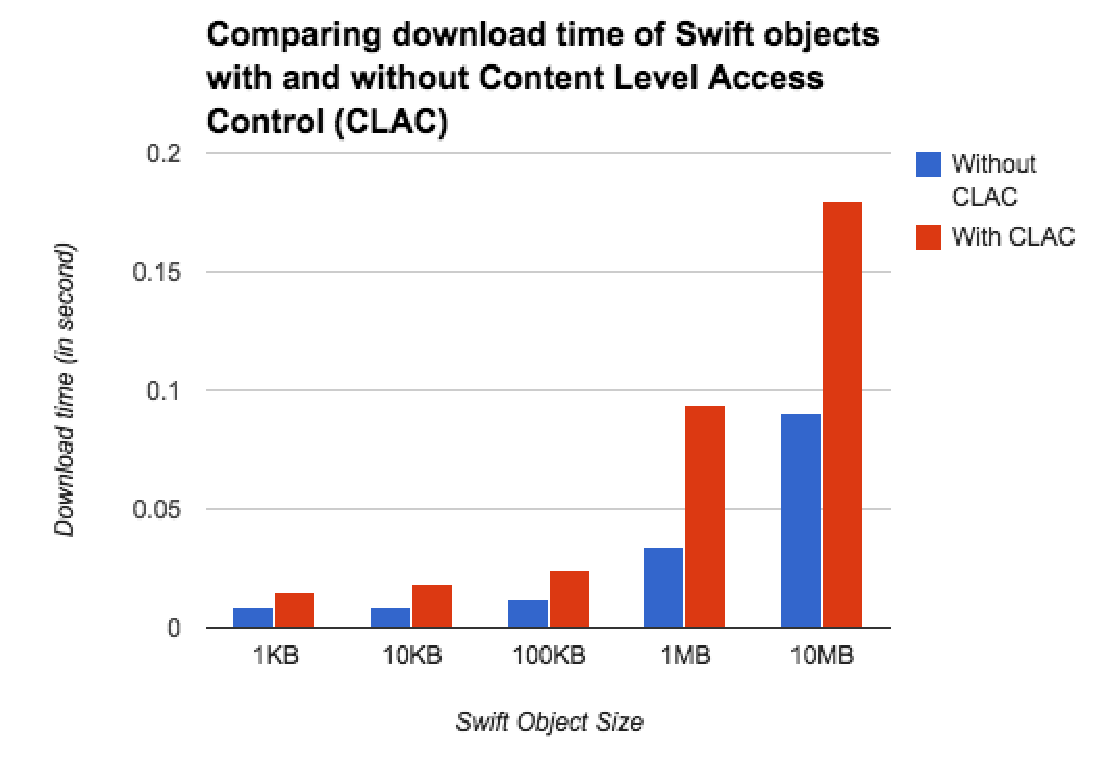
\includegraphics[width=0.5\textwidth]{CODASPY15/performance.eps}
 \caption{ Performance of our Implementation}
   \label{fig:performance}
\end{figure}

%\section{Related Work}
%There have  been very few works for access control of JSON data, although JSON and XML data are very similar and lots of works has been done at the content level for XML data \cite{ bertino2000specifying,damiani2002fine}.  Additionally there are prior works that apply object labels at the content level \cite{adam2002content} for access control purposes. But, to the best of our knowledge, applying content level access control for the application context of OpenStack Swift has not yet been  performed. 